\begin{DensePanel}{268mm}{12}{WHAT RETUNING CANNOT CHANGE}
  {\DenseHead Low-frequency moments\par}
  {\DenseSmall With every $k_I$ fixed, the first two moments of the frequency response stay put; any PLL-only retune leaves the differences of bus frequency areas unchanged:\par}
  {\DenseEq\color{IASBlue}\[
    H_{\mathrm{new}}(s)-H_{\mathrm{base}}(s)=O(s^{2}),\qquad \int_0^\infty (f_{\mathrm{new}}-f_{\mathrm{base}})\,dt=0
  \]}
  \vspace{-2mm}
  {\DenseHead A network inertia floor\par}
  \noindent\begin{minipage}[t]{150mm}\vspace{0pt}
    {\DenseSmall\raggedright After a localised step, no local frequency avoids crossing its final value unless\par}
    {\fontsize{25pt}{30pt}\selectfont\color{IASBlue}\[
      m+\kappa>d_0^{2}\,(e_k-c)^{\top}\bar L_k^{\dagger}(e_k-c)
    \]}
    \vspace{1mm}
    {\DenseSmall\raggedright Moving inertia or adding zero-net-energy damping cannot lower it. Two nodes: $\inf m=2\arcsin(P/2)/P$.\par}
  \end{minipage}\hfill%
  \begin{minipage}[t]{122mm}\vspace{0pt}
    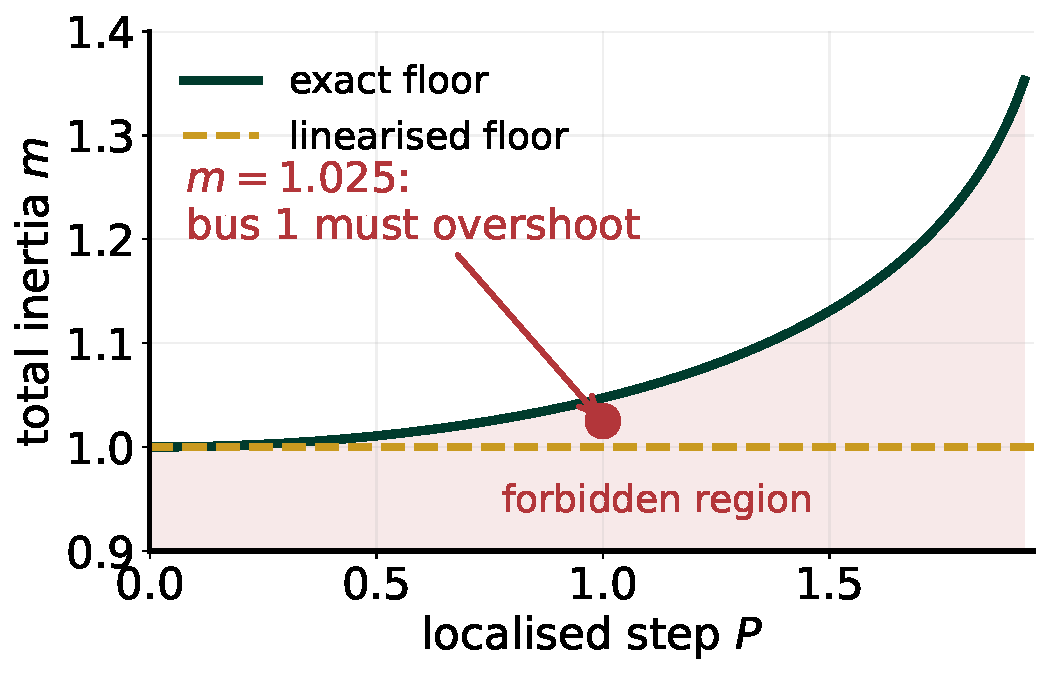
\includegraphics[width=120mm,height=76mm,keepaspectratio]{generated/figures/floor2.pdf}
  \end{minipage}\par
  \vspace{2mm}
  \begin{DenseWords}\textbf{\color{IASGold!65!black}AUDIT\ \ }Retracted: a 94.2\,\% inverter design fails RoCoF (0.513 Hz/s) and frequency (0.589 Hz). Invalid: zero-frequency Schur damping (condition $3\times10^{18}$). Certified: one root cluster over a full share/gain box (485 interval panels). Not claimed: maximum share, optimal mode, superiority over other compensators. Floor: reduced lossless model.\end{DenseWords}
\end{DensePanel}
